%
% File acl2014.tex
%
% Contact: koller@ling.uni-potsdam.de, yusuke@nii.ac.jp
%%
%% Based on the style files for ACL-2013, which were, in turn,
%% Based on the style files for ACL-2012, which were, in turn,
%% based on the style files for ACL-2011, which were, in turn,
%% based on the style files for ACL-2010, which were, in turn,
%% based on the style files for ACL-IJCNLP-2009, which were, in turn,
%% based on the style files for EACL-2009 and IJCNLP-2008...

%% Based on the style files for EACL 2006 by
%%e.agirre@ehu.es or Sergi.Balari@uab.es
%% and that of ACL 08 by Joakim Nivre and Noah Smith

\documentclass[11pt]{article}
\usepackage[utf8]{inputenc}
\usepackage[french]{babel}
\usepackage{acl2014}
\usepackage{times}
\usepackage{url}
\usepackage{latexsym}
\usepackage{graphics}

%\setlength\titlebox{5cm}

% You can expand the titlebox if you need extra space
% to show all the authors. Please do not make the titlebox
% smaller than 5cm (the original size); we will check this
% in the camera-ready version and ask you to change it back.


\title{Agents conversationnels à base de réseaux de neurones artificiels profonds}

\author{Guillaume Chevalier \\
  Université Laval \\ Baccalauréat en génie logiciel \\
  {\tt \small guillaume.chevalier.2@ulaval.ca} \\\And
  Samuel Cabral Cruz \\
  Université Laval \\ Baccalauréat en génie logiciel \\
  {\tt \small samuel.cabral-cruz.1@ulaval.ca} \And
  Nadir Belkhiter (Superviseur) \\
  Université Laval \\ Professeur agrégé \\
  Membre de l’OIQ \\
  {\tt \small nadir.belkhiter@ift.ulaval.ca}}

\date{}

\begin{document}
\maketitle

\begin{abstract}

\end{abstract}

\section{Introduction}


\section{Développement}
\subsection{Traitement d'un intrant vocal}

\subsection{Extraction des composantes de l'intrant et des sources d'information à analyser}
Une fois que la requête de l'utilisateur aura été convertie sous une forme textuelle facilement manipulable par un ordinateur, nous pourrions, dès lors, utiliser le plongement induit par l'étape précédente. Une autre approche consiste à reprendre cette sortie pour ensuite la fournir à une nouvelle structure qui se chargera d'aller extraire de nouvelles composantes qui aideront certainement à obtenir de meilleurs résultats pour la suite du processus. \\

À ce stade, nous devons comprendre que le signal est encore purement textuel et nous n'avons pour seule information qu'une décomposition des mots qui forment la demande reçue. Cependant, les langages sont formés de davantage de subtilités qu'un simple enchaînement de mots les uns après les autres. En effet, chaque mot joue un rôle précis dans la structure de la phrase et apporte une nuance particulière au contexte générale de celle-ci ou encore du texte avec une plus faible portée. C'est exactement ce que les travaux de ... visaient à faire. Ainsi, en ..., ce groupe de chercheurs a fait la publication d'un article détaillant leur approche fondée sur l'utilisation de réseaux de neurones. En plus de faire état de leurs travaux, ce groupe est aussi à l'origine d'outil qui est encore à ce jour considéré comme un incontournable: [WORD2VEC]. \\

Malgré le fait que cet article pour sur les approches neuronales, cet outil a plutôt fait la démonstration que des approches plus simplistes sont parfois plus adaptées. Comme le montre la figure ..., Word2vec se fonde sur la combinaison de deux approches nommées skip-gram et bag of words consistant simplement a. \\

\begin{figure}[ht]
  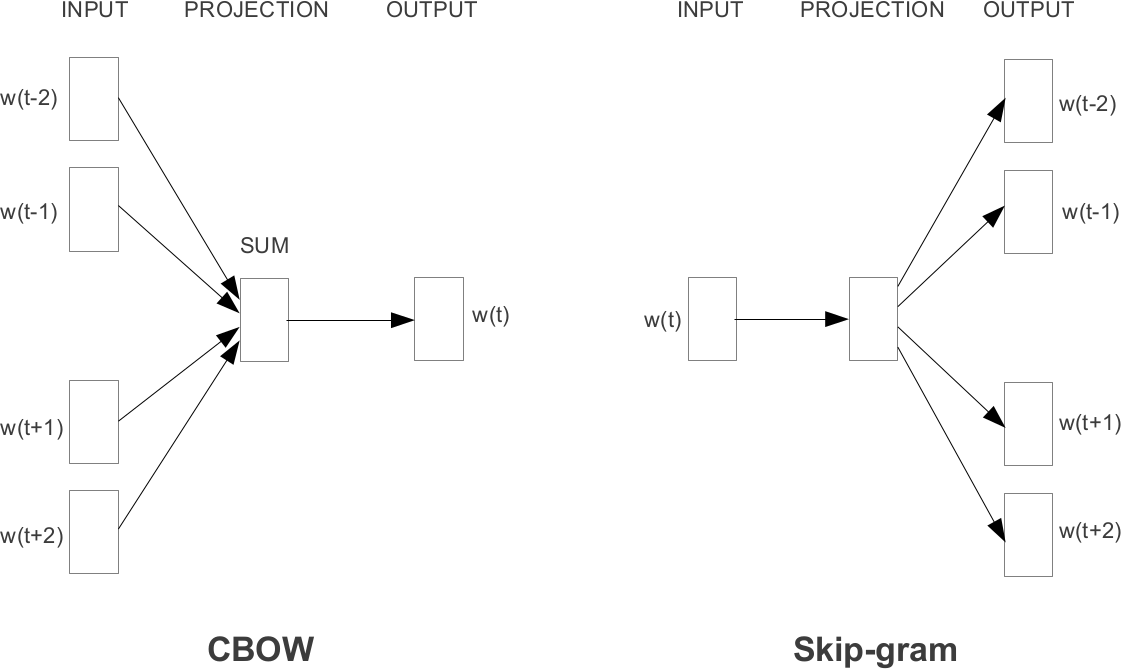
\includegraphics{./../fig/word2vec}
\end{figure}

En fournissant la requête reçue à cet outil, il sera donc possible d'extraire les composantes sémantiques et syntaxiques sous-entendues par cette dernière. Par la suite, ces nouvelles composantes seront combinées à celle que nous avions déjà obtenues à l'étape précédente. En procédant avec cette seconde approche, nous réaliserons certainement un gain majeur au niveau de la performance des prochaines étapes en raison de l'ajout important de dimensionnalités qui fourniront beaucoup plus de flexibilité aux réseaux de neurones suivantes qui devront à leur tour détecter les nuances du langage. À titre d'exemple, lorsqu'un utilisateur demandera à l'assistant si ce dernier peut lui indiquer l'horaire du cinéma le plus prêt de sa position, l'assistant devra comprendre la nuance que ce qui intéresse vraiment l'utilisateur est l'horaire et non pas l'évaluation booléenne de sa capacité à s'acquitter de cette tâche. Par contre, dans le cas où l'utilisateur demanderait à l'assistant si ce dernier peut le connecté à l'Internet, l'assistant devra dans ce cas faire l'évaluation de sa capacité et répondre en par affirmation à notre cher utilisateur. [Référence au transfer learning (TODO)] \\

Mais qu'en est-il de nos sources d'informations? En fait, le processus entier bénéficiera certainement qu'un travail similaire soit fait à ce niveau aussi. Pour ce faire, deux approches s'offrent encore à nous. La première consistant encore une fois à utiliser word2vec et la seconde repose sur le même principe, mais à un niveau supérieur d'abstraction en considérant cette fois l'utilité de chacune des phrases dans le texte plutôt que de se concentrer sur le rôle de chaque mot dans chaque phrase.  \\

Il y a 2 façons d’avoir l’embedding du corpus de texte (ex: tout wikipédia) lequel sera utilisé pour répondre à la question. Word2vec et infersent. Expliquer les niveaux d’emedding de word2vec et infersent (word-level et sentence-level). Plugger ça dans un RNN ou autre chose, tel que vu à la section suivante.

\subsection{Interprêter la requête et cibler le contenu d'intérêt pour y répondre}

\subsection{Formulation d'une réponse à partir de l'information d'intérêt retenur}

\subsection{Retourner la réponse textuelle sous la forme d'un signal audio}

\section*{Conclusion}

\section*{Remerciements}

% include your own bib file like this:
%\bibliographystyle{acl}
%\bibliography{acl2014}

\begin{thebibliography}{}
%Example
\bibitem[\protect\citename{Aho and Ullman}1972]{Aho:72}
Alfred~V. Aho and Jeffrey~D. Ullman.
\newblock 1972.
\newblock {\em The Theory of Parsing, Translation and Compiling}, volume~1.
\newblock Prentice-{Hall}, Englewood Cliffs, NJ.

\end{thebibliography}

\end{document}
